\documentclass[
	a4paper,
	oneside,
	BCOR = 10mm,
	DIV = 12,
	12pt,
	headings = normal,
]{scrartcl}

%%% Length calculations
\usepackage{calc}
%%%

%%% Support for color
\usepackage{xcolor}
\definecolor{lightblue}{HTML}{03A9F4}
\definecolor{red}{HTML}{F44336}
%%%

%%% Including graphics
\usepackage{graphicx}
%%%

%%% Font selection
\usepackage{fontspec}

\setromanfont{STIX Two Text}[
	SmallCapsFeatures = {LetterSpace = 8},
]

\setsansfont{IBM Plex Sans}[
	Scale = MatchUppercase,
]

\setmonofont{IBM Plex Mono}[
	Scale = MatchUppercase,
]
%%%

%%% Math typesetting
\usepackage{amsmath}

\usepackage{unicode-math}
\setmathfont{STIX Two Math}

\usepackage{IEEEtrantools}
%%%

%%% List settings
\usepackage{enumitem}
\setlist[enumerate]{
	label*      = {\arabic*.},
	leftmargin  = *,
	labelindent = \parindent,
	topsep      = 1\baselineskip,
	parsep      = 0\baselineskip,
	itemsep     = 1\baselineskip,
	noitemsep, % override itemsep
}

\setlist[itemize]{
	label*      = {—},
	leftmargin  = *,
	labelindent = \parindent,
	topsep      = 1\baselineskip,
	parsep      = 0\baselineskip,
	itemsep     = 1\baselineskip,
	noitemsep, % override itemsep
}

\setlist[description]{
	font        = {\rmfamily\upshape\bfseries},
	topsep      = 1\baselineskip,
	parsep      = 0\baselineskip,
	itemsep     = 0\baselineskip,
}

%%%

%%% Structural elements typesetting
\setkomafont{pagenumber}{\rmfamily\upshape}
\setkomafont{disposition}{\rmfamily\bfseries}

% Sectioning
\RedeclareSectionCommand[
	beforeskip = -1\baselineskip,
	afterskip  = 1\baselineskip,
	font       = {\normalsize\bfseries\scshape},
]{section}

\RedeclareSectionCommand[
	beforeskip = -1\baselineskip,
	afterskip  = 1\baselineskip,
	font       = {\normalsize\bfseries\itshape},
]{subsection}

\RedeclareSectionCommand[
	beforeskip = -1\baselineskip,
	afterskip  = 1\baselineskip,
	font       = {\normalsize\bfseries},
]{subsubsection}

\RedeclareSectionCommand[
	beforeskip = -1\baselineskip,
	afterskip  = -0.5em,
	font       = {\normalsize\mdseries\scshape\addfontfeatures{Letters = {UppercaseSmallCaps}}},
]{paragraph}
%%%

%%% Typographic enhancements
\usepackage{microtype}
%%%

%%% Language-specific settings
\usepackage{polyglossia}
\setmainlanguage{ukrainian}
\setotherlanguages{english}
%%%

%%% Captions
\usepackage{caption}
\usepackage{subcaption}

%\DeclareCaptionLabelFormat{closing}{#2)}
%\captionsetup[subtable]{labelformat = closing}

%\captionsetup[subfigure]{labelformat = closing}

\captionsetup[table]{
	aboveskip = 0\baselineskip,
	belowskip = 0\baselineskip,
}

\captionsetup[figure]{
	aboveskip = 1\baselineskip,
	belowskip = 0\baselineskip,
}

\captionsetup[subfigure]{
	labelformat = simple,
	labelformat = brace,
}
%%%

%%% Hyphenated ragged typesetting
\usepackage{ragged2e}
%%%

%%% Table typesetting
\usepackage{booktabs}
\usepackage{longtable}

\usepackage{multirow}

\usepackage{array}
\newcolumntype{v}[1]{>{\RaggedRight\arraybackslash\hspace{0pt}}p{#1}}
\newcolumntype{b}[1]{>{\Centering\arraybackslash\hspace{0pt}}p{#1}}
\newcolumntype{n}[1]{>{\RaggedLeft\arraybackslash\hspace{0pt}}p{#1}}
%%%

%%% Drawing
\usepackage{tikz}
\usepackage{tikzscale}
\usetikzlibrary{positioning}
\usetikzlibrary{arrows.meta} % Stealth arrow tips
%%%

%%% SI units typesetting
\usepackage{siunitx}
\sisetup{
	output-decimal-marker = {,},
	exponent-product      = {\cdot},
	inter-unit-product    = \ensuremath{{} \cdot {}},
	per-mode              = symbol,
}
%%%

%%% Framing code listings
\usepackage{tcolorbox}
\tcbuselibrary{breakable}
\tcbuselibrary{minted}
\tcbuselibrary{skins}

\newtcblisting[
	auto counter,
	list inside, 
	number within = section,
]{listingpython}[3][]{%
	minted language = python,
	minted style    = bw,
	minted options  = {
		linenos,
		tabsize = 4,
		breaklines,
		% breakanywhere,
		fontsize = \footnotesize,
		autogobble
	},
	%
	% empty,
	sharp corners,
	colframe         = black,
	colback          = black!0,
	leftrule         = 0em,
	rightrule        = 0em,
	toprule          = 1pt, % orig = 0pt
	bottomrule       = 1pt, % orig = 0pt
	titlerule        = 0.5pt,
	colbacktitle     = black!0,
	coltitle         = black,
	toptitle         = 0.3em,
	bottomtitle      = 0.1em,
	borderline north = {1pt}{0pt}{black},
	borderline south = {1pt}{0pt}{black},
	before skip      = \intextsep,
	after  skip      = \intextsep,
	title            = {Лістинг \thetcbcounter: #2},
	list entry       = {\protect\numberline{\thetcbcounter}#2},
	left = 0em,
	right = 0em,
	%
	listing only,
	breakable,
	%
	label = {#3},
	%
	#1
}

\newtcbinputlisting[auto counter, list inside, number within = section]{\inputpython}[4][]{%
	minted language = python,
	minted style    = bw,
	minted options  = {
		linenos,
		tabsize = 4,
		breaklines,
		breakbytokenanywhere,
		fontsize = \footnotesize,
	},
	%
	% empty,
	sharp corners,
	colframe         = black,
	colback          = black!0,
	leftrule         = 0em,
	rightrule        = 0em,
	toprule          = 0pt, % orig = 0pt
	bottomrule       = 0pt, % orig = 0pt
	titlerule        = 0.5pt,
	colbacktitle     = black!0,
	coltitle         = black,
	toptitle         = 0.3em,
	bottomtitle      = 0.1em,
	borderline north = {1pt}{0pt}{black},
	borderline south = {1pt}{0pt}{black},
	before skip      = \intextsep,
	after  skip      = \intextsep,
	title            = {Лістинг \thetcbcounter: #3},
	list entry       = {\protect\numberline{\thetcbcounter}#3},
	left = 0em,
	right = 0em,
	%
	listing file={#2},
	listing only,
	breakable,
	%
	label = {#4},
	%
	#1
}

% Customize minted
\usepackage{minted}
\setmintedinline{
	style = bw,
	breaklines,
}

% Customize minted line numbers
\renewcommand{\theFancyVerbLine}{\ttfamily\scriptsize\arabic{FancyVerbLine}}

%%%

%%% Links and hyperreferences
\usepackage{hyperref}
\hypersetup{
	bookmarksnumbered = true,
	colorlinks      = false,
	linkbordercolor = red,
	urlbordercolor  = lightblue,
	pdfborderstyle  = {/S/U/W 1.5},
}
%%%

%%% Length adjustments
% Set baselineskip, default is 14.5 pt
\linespread{1.068966} % ~15.5 pt
\setlength{\emergencystretch}{2em}
\setlength{\parindent}{1.5em}
\newlength{\gridunitwidth}
\setlength{\gridunitwidth}{\textwidth / 12}
%%%

%%% Custom commands
\newcommand{\allcaps}[1]{{\addfontfeatures{LetterSpace = 8, Kerning = Off}#1}}
\newcommand{\filename}[1]{\texttt{#1}}
\newcommand{\progname}[1]{\texttt{#1}}
\newcommand{\modulename}[1]{\texttt{#1}}

\newcommand{\schel}[1]{\textit{#1}}
%%%

%%% Custom math commands
\newcommand{\longvar}[1]{\mathit{#1}}
\DeclareMathOperator{\MTF}{MTF}
%%%

%%% Custom units
\DeclareSIUnit{\px}{пкс}
%%%

\begin{document}

\begin{titlepage}
		\begin{center}
			Міністерство освіти і~науки України\\
			Національний авіаційний університет\\
			Навчально-науковий інститут комп'ютерних інформаційних технологій\\
			Кафедра комп'ютеризованих систем управління

			\vspace{\fill}
				Лабораторна робота №6\\
				з~дисципліни «Діагностика та~експлуатація комп'ютера»\\
				на~тему «Вимірювання роздільної здатності \textenglish{WEB}-камери»\\

			\vspace{\fill}

			\begin{flushright}
				Виконав:\\
				студент \allcaps{ННІКІТ}\\
				групи СП-325\\
				Клокун В.\,Д.\\
				Перевірила:\\
				Голего Н.\,М.
			\end{flushright}

			Київ 2019
		\end{center}
	\end{titlepage}

	\section{Мета роботи}
		Знайомство з~методиками визначення основних характеристик \textenglish{WEB}-камер за~допомогою тестування та~практичне визначення графіка модуляційної передавальної функції~(\textenglish{MTF}). 

	\section{Хід~роботи}
		Готуємо робоче місце для~зйомки. Для~цього прикріплюємо тестову таблицю в~центр аркушу~\textenglish{A4}. Фотографуємо тестову таблицю. В~результаті отримаємо зображення. Завантажуємо отримане зображення в~графічний редактор та~коригуємо рівні так, щоб~білі лінії на~зображенні були максимально білими, а~чорні~— чорними. Зберігаємо остаточне зображення у~форматі~\textenglish{JPG} з~шириною~\SI{1000}{\px}.

		Тепер аналізуємо отримане зображення. Для~цього відкриваємо збережене зображення в~програмі~\textenglish{Pixel Profile} і~обираємо область для~аналізу. Для~цього проводимо лінію у~верхній синусоїдальній частині зображення~(рис.~\ref{fig:pixelprofile-image}).
		\begin{figure}[!htbp]
			\centering
			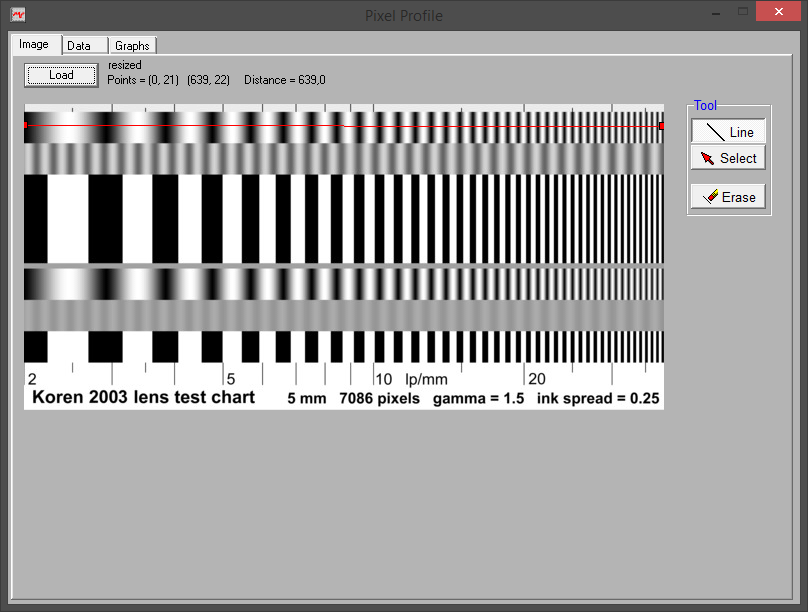
\includegraphics[height=10\baselineskip]{./assets/y03s02-pcdiag-lab-06-p00-pixelprofile.png}
			\caption{Програма \textenglish{Pixel Profile}: вибір області для~аналізу}
			\label{fig:pixelprofile-image}
		\end{figure}

		Після того, як~програма проаналізує обрану область, вона виведе результати аналізу у~відповідних вкладках~(рис.~\ref{subfig:pixelprofile-data}, \ref{subfig:pixelprofile-graphs}).

		\begin{figure}[!htbp]
			\centering
			\begin{subfigure}[t]{\columnwidth / 2}
				\centering
				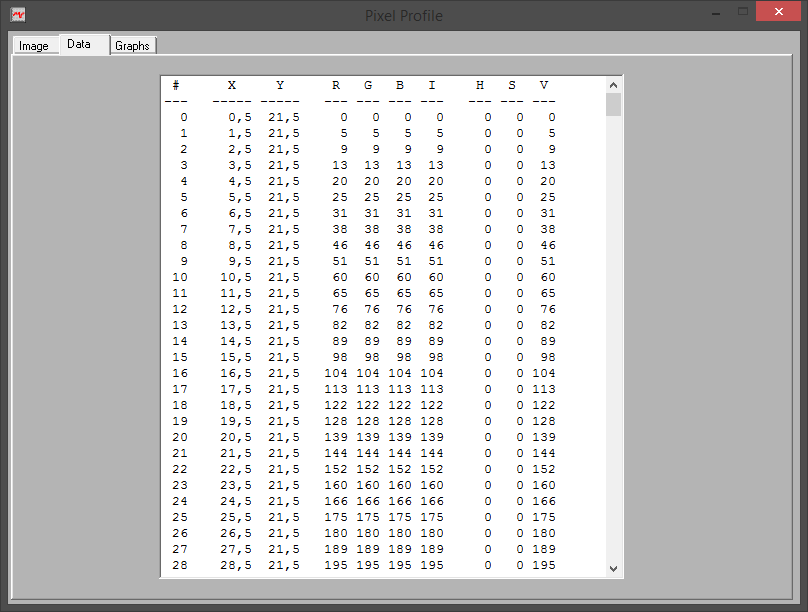
\includegraphics[height=10\baselineskip]{./assets/y03s02-pcdiag-lab-06-p01-pixelprofile-data.png}
				\caption{}
				\label{subfig:pixelprofile-data}
			\end{subfigure}%
			\begin{subfigure}[t]{\columnwidth / 2}
				\centering
				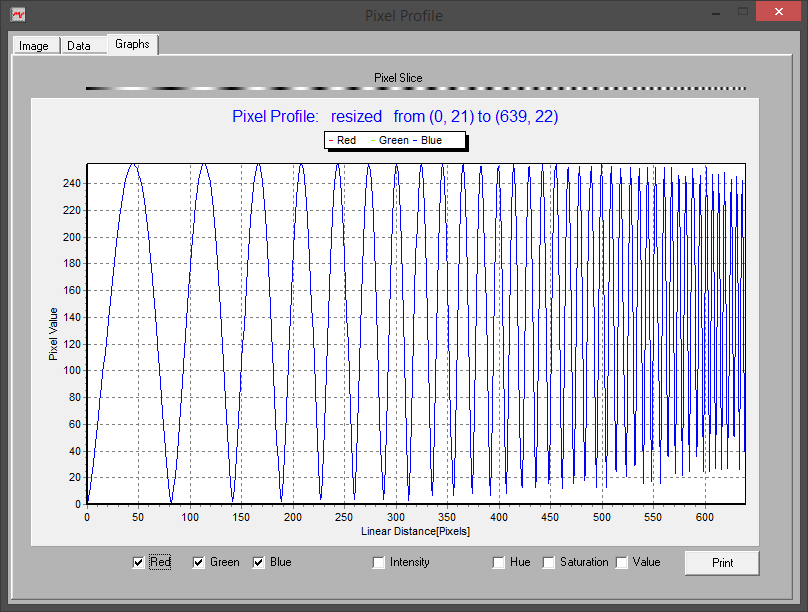
\includegraphics[height=10\baselineskip]{./assets/y03s02-pcdiag-lab-06-p02-pixelprofile-graphs.png}
				\caption{}
				\label{subfig:pixelprofile-graphs}
			\end{subfigure}
			\caption{Програма~\textenglish{Pixel Profile}: \subref{subfig:pixelprofile-data}~— вкладка даних~— результатів аналізу, \subref{subfig:pixelprofile-graphs}~— вкладка графіків~— результатів аналізу}
			\label{fig:pixelprofile}
		\end{figure}

		Отримавши результати аналізу зображення, виділяємо потрібні, а~саме номер піксела і~його яскравість. Далі обчислюємо значення частоти~$f_i$ для~кожної точки~$i$ за~такою формулою:
		\begin{IEEEeqnarray*}{rCl}
			f_{i} =
			2 \cdot
			\exp \left(
				\frac{N_{i}}{N_{\text{max}}}
				\cdot
				\left(
					\ln \left( F_{\text{max}} \right)
					- \ln \left( F_{\text{min}} \right)
				\right)
			\right),
		\end{IEEEeqnarray*}
		де~$N_i$~— порядковий номер поточної точки, $N_{\text{max}}$~— порядковий номер останньої точки, $F_{\text{min}}$ і~$F_{\text{max}}$~— мінімальне і~максимальне значення частоти ліній, охоплених для~аналізу в~\textenglish{Pixel Profile}. Зберігаємо отриманий результат.

		Завантажуємо проаналізовані значення у~програму~\textenglish{Advanced Grapher}, налаштовуємо параметри бажаного графіка і~запускаємо побудову. В~результаті отримали графік яскравості кожної точки аналізованої області~(рис.~\ref{fig:agrapher-plot-raw}).

		\begin{figure}[!htbp]
			\centering
			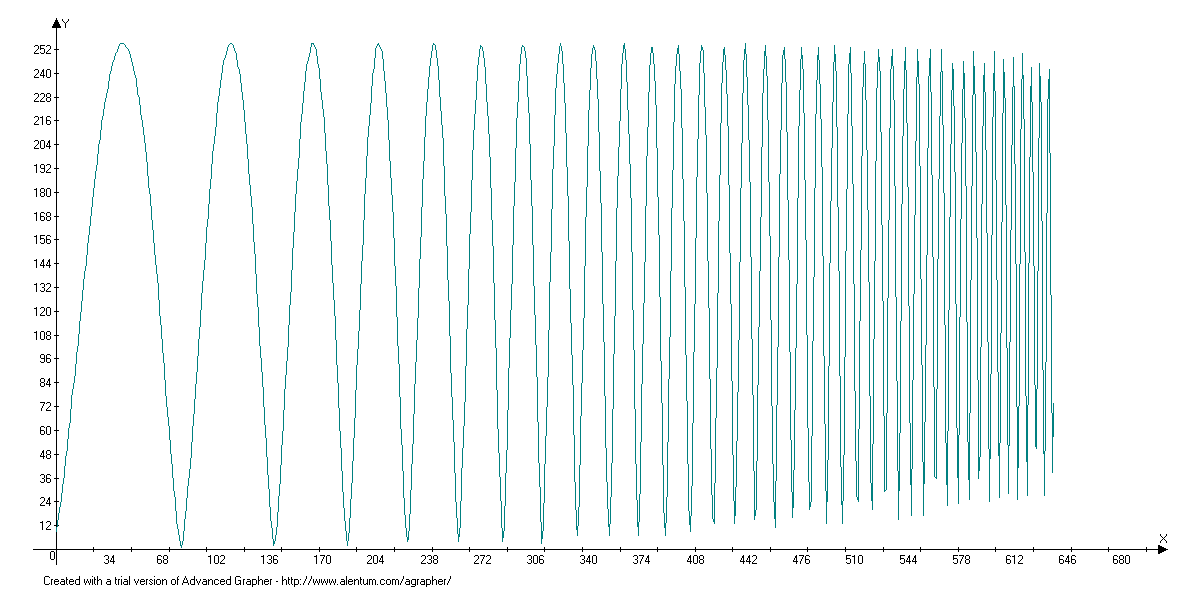
\includegraphics[height = 14\baselineskip]{./assets/y03s02-pcdiag-lab-06-p03-agr-plot-raw.png}
			\caption{Графік яскравості проаналізованих точок зображення}
			\label{fig:agrapher-plot-raw}
		\end{figure}

		На~отриманому графіку встановлюємо точки, що~приблизно обмежують графік знизу і~зверху. В~програмі~\textenglish{Advanced Grapher} на~основі заданих точок запускаємо побудову кривих на~основі поліному 4-го~порядку. Назвемо ці~криві~$y_{\text{low}}(x)$, $y_{\text{high}}(x)$. Після того, як~криві будуть визначені, вони з'являться на~графіку~(рис.~\ref{fig:agrapher-plot-asymptotes}).

		\begin{figure}[!htbp]
			\centering
			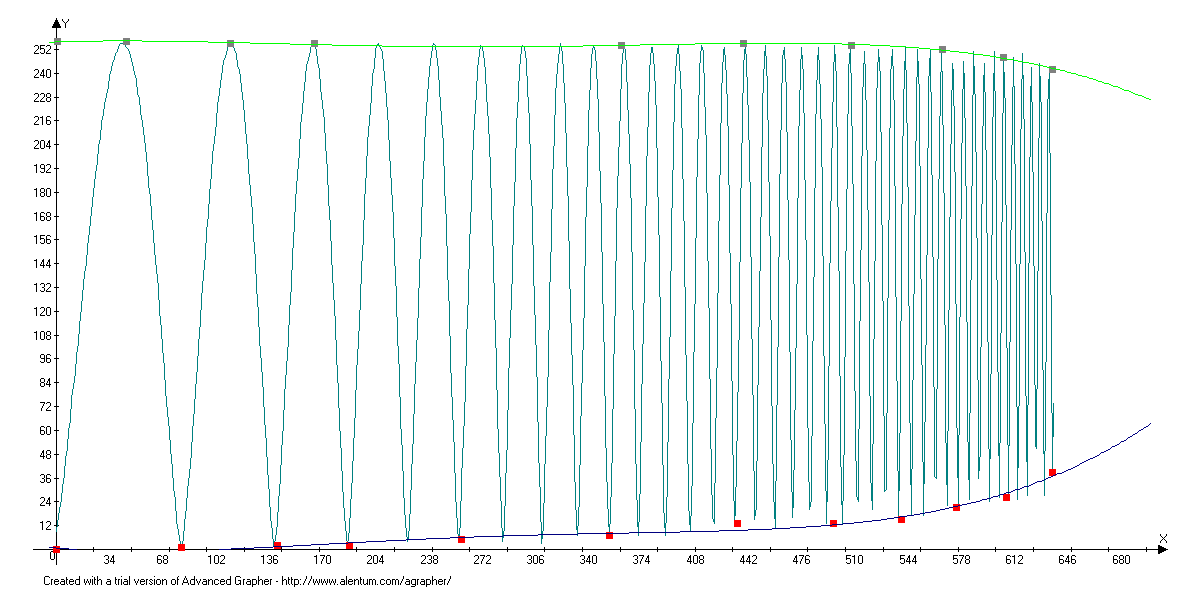
\includegraphics[height = 11\baselineskip]{./assets/y03s02-pcdiag-lab-06-p04-agr-plot-asymptotes.png}
			\caption{Графік яскравості проаналізованих точок зображення з~обмежуючими кривими}
			\label{fig:agrapher-plot-asymptotes}
		\end{figure}

		За~допомогою функції~«\textenglish{Value Table}» програми~\textenglish{Advanced Grapher} обчислюємо значення точок отриманих обмежуючих кривих та~зберігаємо їх~у~відповідні файли. На~основі збережених значень розраховуємо значення~модуляційної передавальної функції~$\MTF$ за~такою формулою:
		\begin{IEEEeqnarray*}{rCl}
			\MTF(x) =
			\frac{
				y_{\text{high}}(x) - y_{\text{low}}(x)
			}{
				y_{\text{high}}(x) + y_{\text{low}}(x)
			},
		\end{IEEEeqnarray*}
		де~$y_{\text{low}}(x)$ і~$y_{\text{high}}(x)$~— значення функцій нижньої і~верхньої обмежуючих кривих для~точки~$x$.

		На~основі отриманих значень~$\MTF(x)$ в~програмі~\textenglish{Advanced Grapher} будуємо графік модуляційної передавальної функції~(рис.~\ref{fig:agrapher-plot-mtf}).

		\begin{figure}[!htbp]
			\centering
			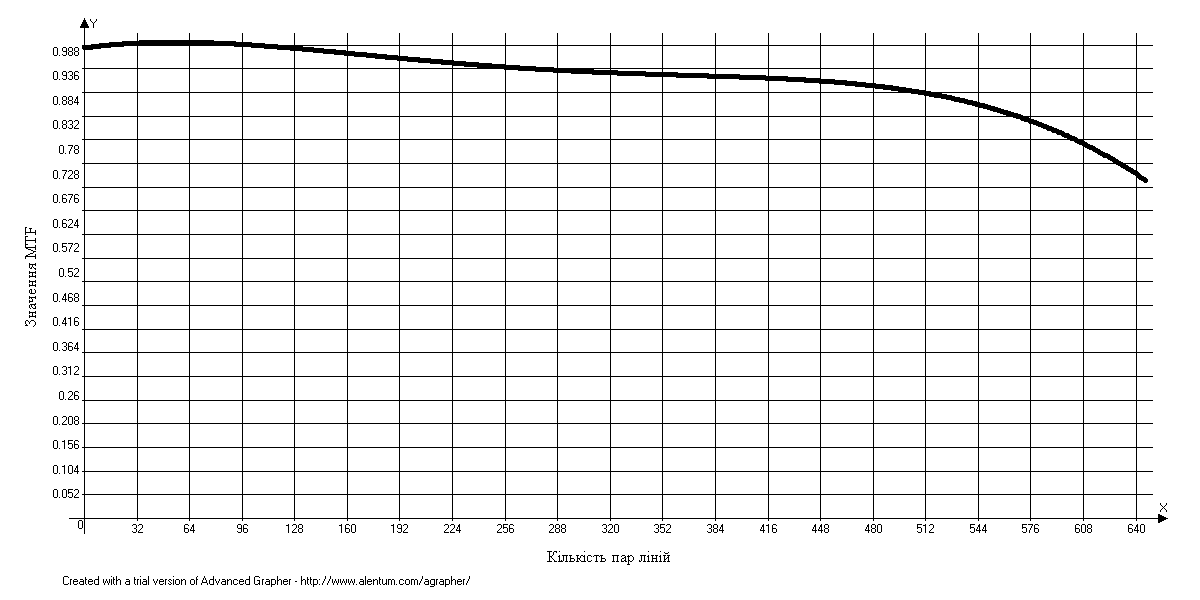
\includegraphics[height = 11\baselineskip]{./assets/y03s02-pcdiag-lab-06-p05-agr-plot-mtf.png}
			\caption{Графік модуляційної передавальної функції~$\MTF(x)$}
			\label{fig:agrapher-plot-mtf}
		\end{figure}


	\section{Висновок}
		Виконуючи дану лабораторну роботу, ми~ознайомились з~методиками визначення основних характеристик веб-камер за~допомогою тестування та~практично визначили графік модуляційної передавальної функції.

\end{document}

